%% ------------------------------------------------------------------------- %%
\chapter{Hash Tables}
\label{cap:Hash Tables}

\begin{itemize}
\item Define hash table and its operations
\item Open Addressing Strategies (Linear Probing, Quadratic Probing, ...)
\item Chaining Strategy (Simple Chaining, Move-to-front ...)
\item Load factor and resizing/rehashing the table
\end{itemize}


Hash tables or hash maps is one of the most used applications of hash functions. It is actually so used in computer science that is almost impossible to talk about one without mentioning the other. This data structure consists in associating a \textit{key} to a \textit{value} in a table. That is, given a \textit{key}, it can retrieve the correct \textit{value} for it.

This data structure is usually considered very useful among software engineers and computer scientists, although it usually has a linear worst case cost for retrieving, inserting and deleting a key a value pair. That is because it has a constant average and amortized cost for those operations.

Moreover, when talking about hash tables we have the problem of key collision, that is when two keys maps to the same hash value. To solve that problem, we have several techniques that envolves different tradeoffs. Those techniques are usually divided into two main categories, open addressing and separate chaining. Other problem to consider regarding this data structure is when to resize the hash table, to minimize the chance of collision and the use o memory.

It is also important to notice that hash tables have applications in different areas of computer science also, like compilers, caches and database indexing.


\begin{figure}[h!]
  \centering
  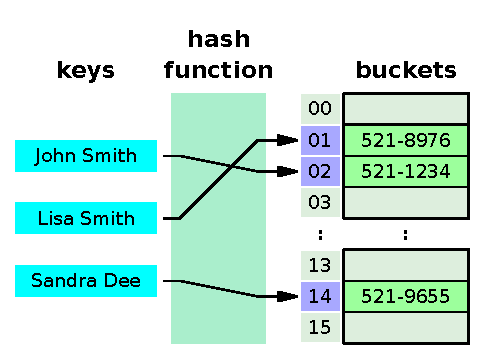
\includegraphics[width=12cm]{figuras/hash-table.pdf}
  \caption{Example of a hash table from string to string, more specifically name to number}
\end{figure}
